\section{实验}

\begin{table*}[!h]
\centering
\resizebox{\textwidth}{!}{%
\begin{tabular}{lcccccccccc}
\toprule
\textbf{模型} & \textbf{Teams} & \textbf{CSM} & \textbf{Email} & \textbf{ITSM} & \textbf{Calendar} & \textbf{HR} & \textbf{Drive} & \textbf{Hybrid} & \textbf{不可行} & \textbf{平均}\\
\midrule
\rowcolor{gray!15} \multicolumn{11}{c}{\textit{闭源模型}} \\
Claude Opus 4.5 \citep{anthropic2025sonnet45} & 50.0 & 34.2 & {51.9} & 23.8 & \textbf{43.2} & \textbf{32.1} & 49.5 & \textbf{30.7} & 50.0 & \textbf{37.4} \\
Gemini-3-Flash \citep{comanici2025gemini25pushingfrontier} & 47.3 & 35.0 & 44.3 & \textbf{28.5} & 30.5 & 12.6 & 49.7 & 24.2 & 38.5 & 31.9 \\
GPT-5.2 (High) \citep{openai2025gpt5} & 31.0 & 34.8 & 51.0 & 21.7 & 38.5 & 25.0 & 40.0 & 22.2 & 50.0 & 31.8 \\
Claude Sonnet 4.5 \citep{anthropic2025sonnet45} & \textbf{51.0} & 16.7 & 51.3 & 17.6 & 34.6 & 21.6 & \textbf{52.1} & 28.1 & 46.2 & 30.9 \\
GPT-5 \citep{openai2025gpt5} & 26.3 & \textbf{36.4} & 49.0 & 18.9 & 41.3 & 17.9 & 34.0 & 23.5 & 50.5 & 29.8 \\
Gemini-3-Pro \citep{comanici2025gemini25pushingfrontier} & 43.0 & 27.7 & 33.6 & 22.2 & 28.8 & 12.5 & 46.7 & 22.9 & 50.0 & 28.0 \\
GPT-5.2 (Low) \citep{openai2025gpt5} & 25.0 & 21.2 & 43.3 & 6.7 & 28.9 & 13.0 & 26.7 & 20.9 & \textbf{53.9} & 21.9 \\
GPT-5-Mini \citep{openai2025gpt5} & 25.7 & 15.8 & 47.4 & 8.9 & 28.8 & 10.7 & 23.8 & 22.5 & 47.4 & 21.3 \\
Gemini-2.5-Pro \citep{comanici2025gemini25pushingfrontier} & 39.3 & 11.6 & 31.1 & 13.9 & 12.5 & 4.9 & 27.0 & 19.6 & 34.7 & 18.2 \\
\rowcolor{gray!15} \multicolumn{11}{c}{\textit{开源模型}} \\
DeepSeek-V3.2 (High)~\citep{deepseekai2024deepseekv3technicalreport} & 37.0 & 14.1 & 47.1 & 16.1 & 21.2 & 16.3 & 35.2 & 22.9 & 53.8 & 24.5 \\
GPT-OSS-120B (High)~\citep{openai2025gptoss120bgptoss20bmodel} & 32.0 & 16.3 & 42.3 & 6.1 & 35.6 & 16.3 & 41.0 & 19.6 & 50.0 & 23.7 \\
DeepSeek-V3.2 (Medium)~\citep{deepseekai2024deepseekv3technicalreport} & 35.7 & 15.4 & 45.8 & 9.6 & 21.5 & 15.0 & 27.6 & 22.9 & 40.0 & 22.3 \\
Kimi-K2-Thinking~\citep{kimiteam2025kimik2openagentic} & 30.0 & 7.1 & 51.0 & 12.2 & 15.4 & 8.2 & 39.6 & 15.7 & 30.5 & 19.5 \\
Qwen3-30B (Think)~\citep{qwen3} & 22.0 & 5.4 & {51.9} & 6.7 & 18.3 & 7.6 & 25.7 & 15.7 & 36.8 & 16.8 \\
Qwen3-235B (Inst.)~\citep{qwen3} & 28.0 & 4.7 & 38.1 & 9.3 & 15.7 & 7.8 & 23.8 & 17.7 & 30.5 & 16.1 \\
Qwen3-4B (Think)~\citep{qwen3} & 24.0 & 3.8 & 38.4 & 5.6 & 5.8 & 7.1 & 21.9 & 15.8 & 31.6 & 13.7 \\
\bottomrule
\end{tabular}%
}
\caption{\ours{} 上的总体任务完成性能。我们报告各模型在预言式工具模式下、按领域划分的成功完成任务百分比。仅当所有以结果为中心的验证检查均通过时，任务才被视为成功。}
\label{tab:main_results}
\end{table*}


\subsection{基线}
\label{subsec:baselines}

我们评估了一组多样化基线，覆盖闭源前沿模型、开源推理模型与非推理模型。所有智能体均在统一接口下评测，使用相同的任务指令、工具定义、沙箱环境和评估协议。除非另有说明，智能体都在\textit{预言式工具}设置下运行，即假设一个完美检索器为智能体提供正确工具集。这样可将评测聚焦于规划和执行本身，无需显式发现工具。我们还通过增加可用工具数量进行消融，以分析工具集大小如何影响性能。我们采用标准的 ReAct 式推理和工具执行循环，它已被证明在智能体设置中有效~\cite{yao2022react}。闭源模型包括 Claude~4.5~\citep{anthropic2025sonnet45, anthropic2025opus45} 的 Opus 和 Sonnet 变体、GPT~\citep{openai2025gpt5} 的 5.2 High、5.2 Low、5 和 5-Mini 变体，以及 Gemini~\citep{comanici2025gemini25pushingfrontier} 的 3-Pro、3-Flash 和 2.5-Pro 变体；开源模型包括 Kimi-K2-Thinking~\citep{kimiteam2025kimik2openagentic}、DeepSeek-V3.2~\citep{deepseekai2024deepseekv3technicalreport}、GPT-OSS-120B（Medium）~\citep{openai2025gptoss120bgptoss20bmodel}，以及 Qwen3~\citep{qwen3} 的 235B Inst.、30B Think 和 4B Think 变体。

\subsection{评估指标}
我们以 pass@1 任务完成率评估模型：仅当模型在满足所有给定约束的同时完成全部任务要求时，得分才为 1。任务完成由基准策划过程中主题专家（SME）手写的 SQL 验证器执行验证。
我们将三次运行的 pass@1 平均值作为主要指标，以降低方差，因为它刻画端到端任务成功。我们也测量验证器级成功率；该指标可细致反映成功验证检查的平均数量，但它可能具有误导性：智能体可能通过平凡轨迹片段的验证器（例如初始设置），却在核心任务逻辑、系统合规要求或副作用检查上失败。因此，pass@1 对现实中智能体效用的评估更准确。

\subsection{结果}

\paragraph{模型在不同领域中的表现如何？}
总体而言，Claude Opus~4.5 达到最佳平均任务完成率（37.4\%），并在多种工作流中表现突出：它在 Email（51.9\%）、Calendar（43.2\%）、HR（32.1\%）和 Hybrid（30.7\%）上领先。Gemini-3-Flash 是总体第二名（31.9\%），并在服务与运维管理工作流 ITSM 上居首（28.5\%）。Claude Sonnet~4.5（30.9\%）在协作和以文档为中心的工作流上仍然强劲，分别在 Teams（51.0\%）和 Drive（52.1\%）上领先。GPT-5 则呈现更具领域特异性的峰值，在 CSM 上最高（36.4\%）。整体上，开源模型仍落后于闭源系统；最强开源模型 DeepSeek-V3.2（High）平均达到 24.5\%，略高于 GPT-OSS-120B（High）的 23.7\%。它们在 CSM、ITSM 和 HR 这类服务、策略和面向人的领域尤为困难。Qwen3-30B（Think）相对于其规模表现出人意料地好，超过了更大的 instruct 变体，并在 Email 上取得很有竞争力的 51.9\%，并列第一。最后，ITSM 和 Hybrid 跨领域工作流是最困难的设置，最佳分数分别仅为 28.5\% 和 30.7\%，突显服务运营和跨领域协调仍是所有模型家族的关键瓶颈。

\paragraph{增加额外工具如何影响性能？}
我们选择总体性能强、成本效益高的 Claude Sonnet 4.5，采用消融实验评估其对工具过载的鲁棒性。我们向预言式工具集加入额外的\textit{干扰}工具（+5、+10 和 +15）。为使该设置尤其困难且能代表现实中的检索错误，我们要求 Claude 检索那些看上去与任务最相关的干扰工具。令人意外的是，性能保持得非常稳定：平均完成率反而平均略增约 $\sim$1.0\%（+5 时为 +0.07\%，+10 时为 +2.35\%，+15 时为 +0.64\%）。唯一另一个显著变化是输出 token 平均增加 4--9\%。这表明模型会利用额外 token 预算仔细筛选并选择合适的工具。这种鲁棒性可能来自 LLM 在工具使用上的广泛训练。因此，我们的结果表明，这些智能体的首要瓶颈并非工具发现，而是任务规划与系统策略遵守。

\paragraph{哪个模型提供最佳性能--成本权衡？}
最佳性能--成本权衡取决于优先考虑绝对质量，还是每美元质量。由 \Cref{fig:cost_vs_preformance} 的 Pareto 前沿可见，Gemini-3-Flash 在闭源模型中提供最强的实用权衡：其单任务成本为 0.03 USD、性能为 31.9\%，以仅为 GPT-5（29.8\%，0.16 USD）和 Claude Sonnet 4.5（30.9\%，0.26 USD）一小部分的成本，取得了更高成功率，成本低 80--90\%。在开源生态中，DeepSeek-V3.2（High）是 Pareto 占优选项，以仅 0.014 USD 达到 24.5\%；紧随其后的是 GPT-OSS-120B（High），以 0.015 USD 达到 23.7\%，二者是总体最具价值的开源选择。Qwen3-235B（Inst.）总体最便宜（0.007 USD），但性能下限显著，仅有 16.1\%。鉴于各系统成功率均低于 40\%，在没有人工监督时它们仍不足以可靠地自治部署。若追求最高绝对可靠性，Claude Opus 4.5 仍是首选（37.4\%），但每任务需付出 0.36 USD 的高昂溢价。

\paragraph{模型拒绝不可行任务的能力如何？}
我们在八个领域中策划了 30 个不可行任务，评估模型是否会对无法满足的请求作出恰当弃权。每个任务平均包含 10 项验证检查，以确保系统中没有副作用。任务通过三种主要机制变得不可行：工具可用性不足、显式策略违规（如日程冲突、数据访问规则等）和资源不可用（如用户未激活、系统处于迁移模式等）。此外，任务采用复合约束，平均每项请求包含 3--4 个约束，模型须评估多个相交条件来判断任务可行性。如表~\ref{tab:main_results} 所示，GPT-5.2（Low）与 DeepSeek-V3.2（High）在弃权且不在系统留下副作用方面最好，分别为 53.9\% 和 53.8\%；GPT-5 为 50.5\%，Claude Opus 4.5、Gemini-3-Pro 和 GPT-OSS-120B（High）等一组模型均为 50.0\%。但所有模型的绝对分数仍远低于生产系统可安全使用的水平。

\begin{figure}[t]
 \centering
 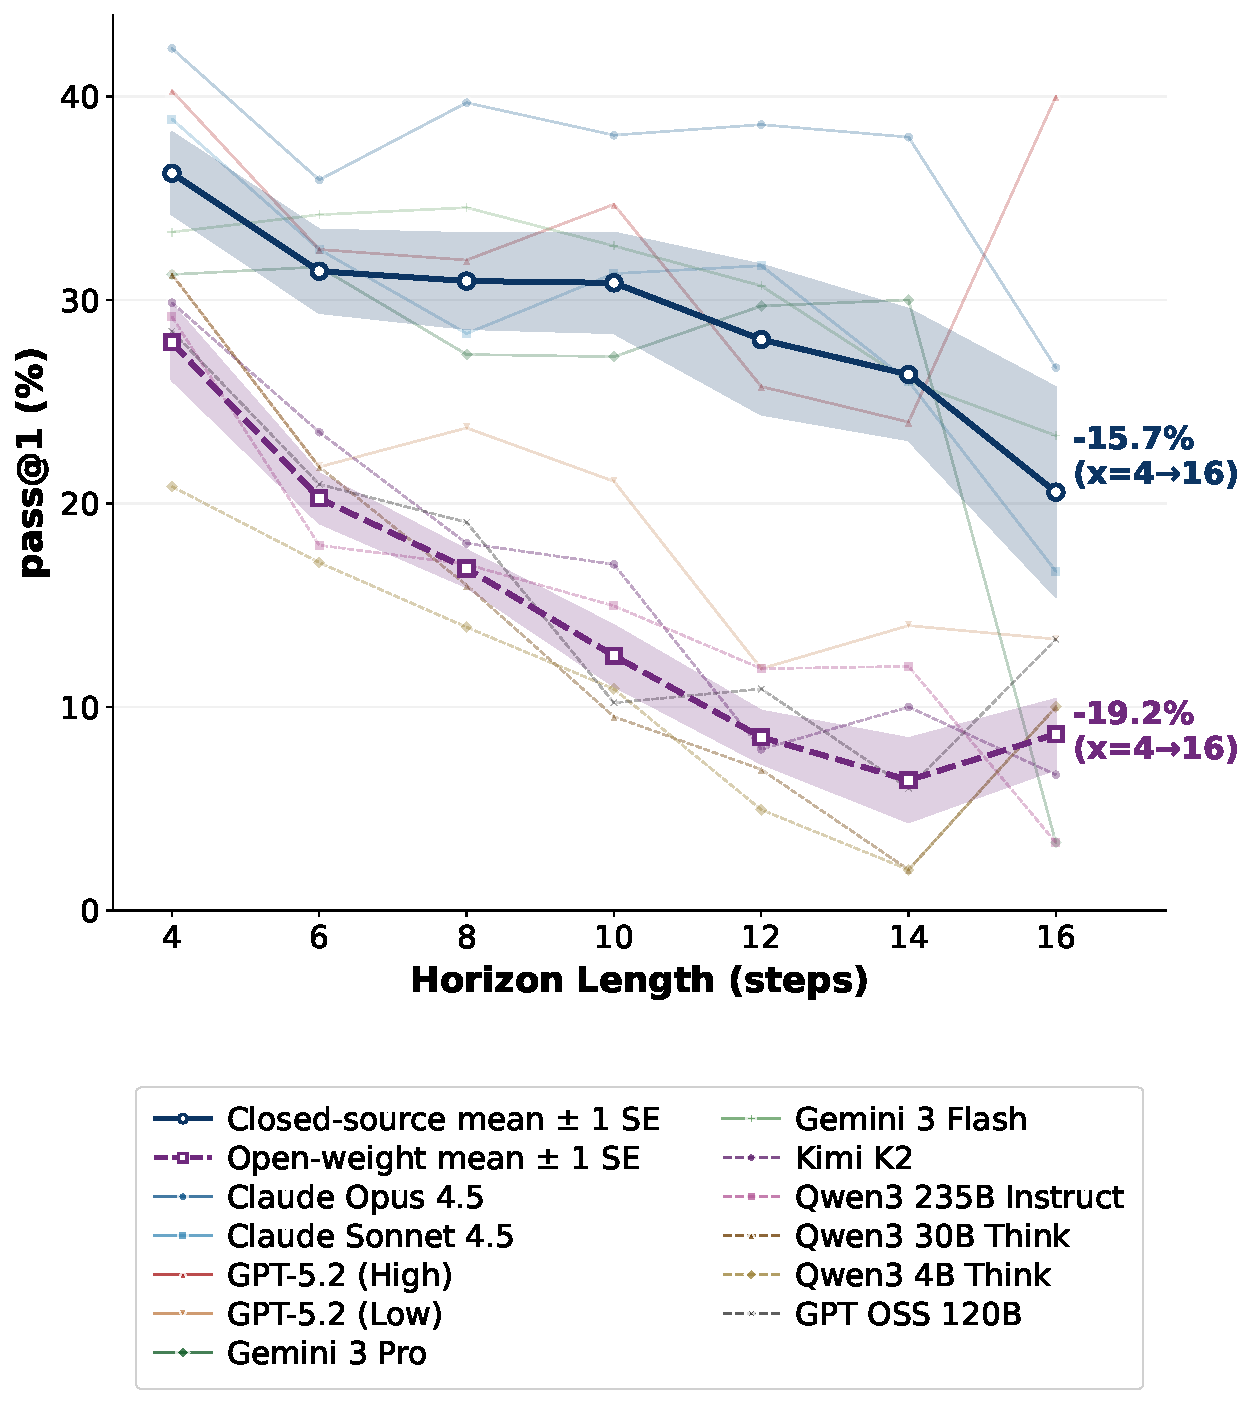
\includegraphics[width=1.0\linewidth]{figures/horizon_trend_single.pdf}
 \caption{\textbf{性能随规划跨度稳定下降。}闭源（实线）和开放权重（虚线）模型在 4--16 个步骤的不同跨度长度上的 Pass@1 准确率。粗线为组均值 $\pm$ 1 个标准误。两组性能均单调下降，开放模型随跨度增长下降更快。}
 \label{fig:performance_by_horizon}
\end{figure}

\begin{figure*}[t]
 \centering
 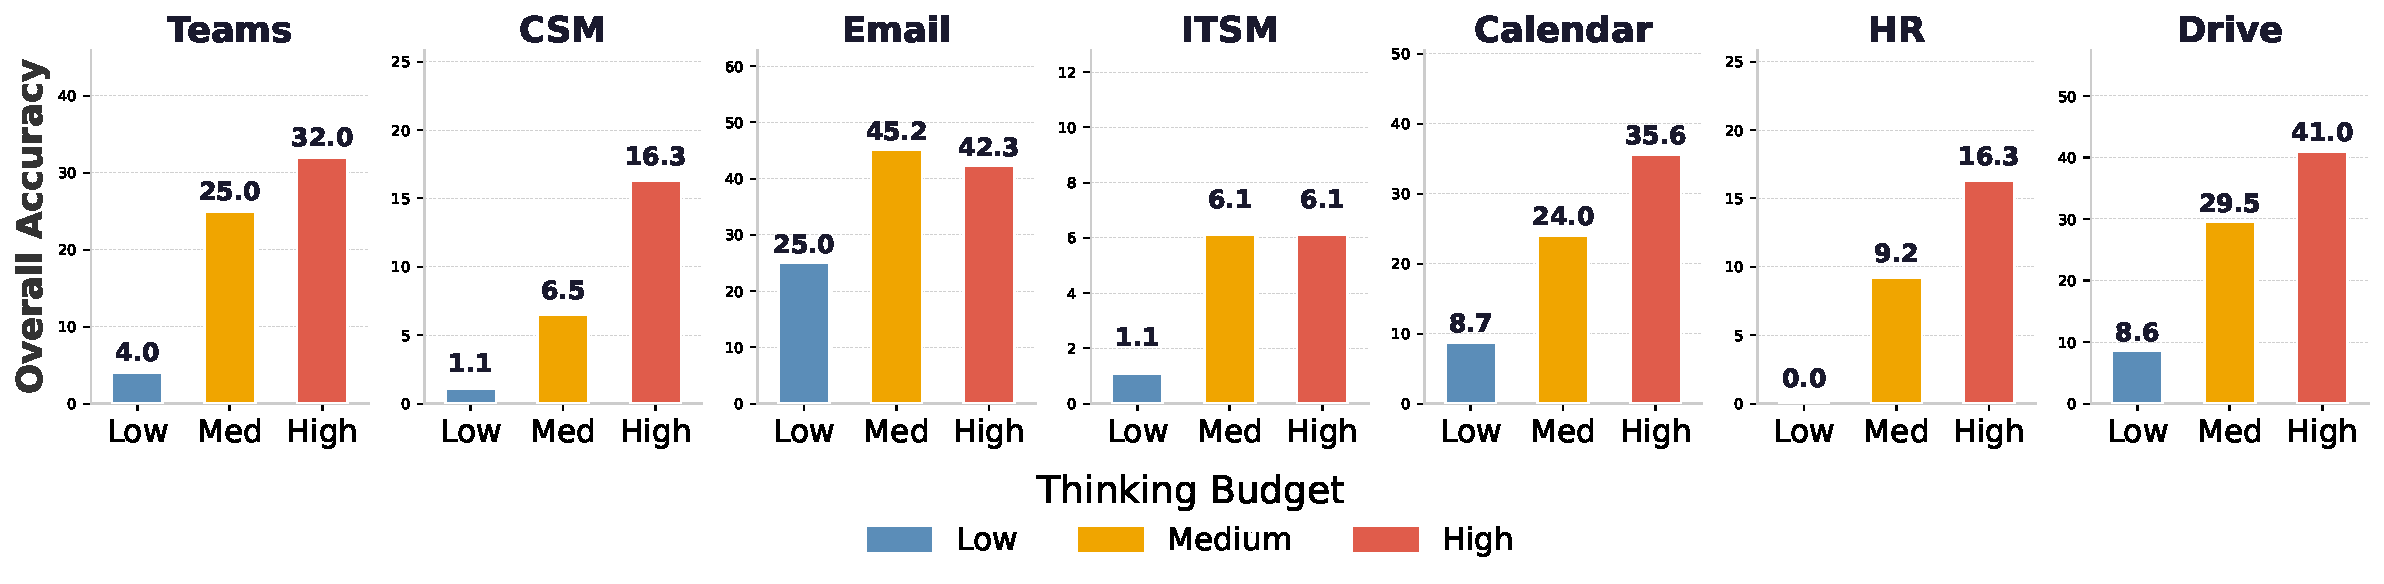
\includegraphics[width=1.0\linewidth]{figures/OSS-Thinking-Performance_pass1.pdf}
 \caption{\textbf{思考预算对性能的影响。}直方图给出 GPT-OSS-120B 模型~\citep{openai2025gptoss120bgptoss20bmodel} 在各领域不同思考预算下的性能。低思考预算下模型表现较差，性能会随思考预算增加而稳步提高。}
 \label{fig:thinking_budget_ablation}
\end{figure*}

\paragraph{性能如何随任务跨度扩展？}
为理解模型能力如何随任务复杂度退化，我们按预期跨度长度对任务分层；该长度与人工编写执行轨迹中的工具执行步数成正比。正如 \Cref{fig:performance_by_horizon} 所示，随着任务跨度增大，所有模型的性能一致衰减，反映出在多步序列中维持推理完整性的累积困难。由 Claude Opus 4.5 领衔的闭源组更有韧性：即使组均值从 4 步时约 35\% 降至 16 步时不足 20\%，它仍保持性能领先。相反，开源组下降更陡，Kimi K2 和 GPT OSS 120B 等模型在最大跨度时趋近 10\% 的成功率。这一近乎普遍的趋势表明，当前模型可处理短至中等长度序列，但长跨度任务中错误快速累积仍是生产环境中自治可靠性的关键障碍。

\paragraph{思考预算如何影响性能？}
我们针对 GPT-OSS-120B 模型~\citep{openai2025gptoss120bgptoss20bmodel}，通过改变\textit{低、中、高}思考预算评估测试时计算的影响。提高思考预算会在几乎所有领域显著改善任务完成（见图~\ref{fig:thinking_budget_ablation}）。在\textit{低}预算下，模型在 CSM（1.1\%）、ITSM（1.1\%）和 HR（0.0\%）等复杂服务与面向人领域中严重受挫，准确率接近零。扩展到\textit{高}预算可释放显著能力：Drive 从 $8.6 \to 41.0$\%，Calendar 从 $8.7 \to 35.6$\%，Teams 从 $4.0 \to 32.0$\%。这种对测试时计算的强依赖说明 \ours{} 的任务执行确实需要复杂推理与规划。但性能扩展并非普遍单调：例如 Email 在\textit{中}预算达到峰值（45.2\%）后略有回落，ITSM 很早就进入平台（$1.1 \to 6.1\% \to 6.1\%$）。这说明仅分配更多思考 token 并不能普遍克服某些工作流中的根本能力瓶颈。

\subsection{进一步分析}

% Custom command for a subtle, smaller improvement value
\newcommand{\up}[1]{\textsubscript{\color{green!50!black}$\uparrow$#1\%}}

\begin{table}[ht]
\centering
\small
\begin{tabular}{@{} l l S[table-format=2.2] @{\,} l S[table-format=2.1] @{\,} l S[table-format=2.2] @{\,} l @{}}
\toprule
\textbf{模型} & \textbf{计划} & \multicolumn{2}{c}{\textbf{CSM}} & \multicolumn{2}{c}{\textbf{ITSM}} & \multicolumn{2}{c}{\textbf{HR}} \\
\midrule
\multirow{2}{*}{Kimi-K2}   & CP & 19.6  & \up{12.5} & 18.1 & \up{5.9}  & 17.2 & \up{9.0} \\
                           & HP & 42.2  & \up{35.1} & 29.1 & \up{16.9} & 34.5 & \up{26.3} \\
\cmidrule(lr){1-8}
\multirow{2}{*}{Qwen3-30B} & CP & 15.2  & \up{9.8}  & 11.7 & \up{5.0}  & 17.9 & \up{10.3} \\
                           & HP & 33.9  & \up{28.5} & 20.9 & \up{14.2} & 33.2 & \up{25.6} \\
\cmidrule(lr){1-8}
\multirow{2}{*}{Qwen3-4B}  & CP & 16.8  & \up{13.0} & 12.2 & \up{6.6}  & 19.6 & \up{12.5} \\
                           & HP & 37.16 & \up{33.4} & 23.3 & \up{17.7} & 36.4 & \up{29.3} \\
\bottomrule
\end{tabular}
\caption{计划条件执行基线。比较使用 Claude 计划（CP）和人工计划（HP）时的性能。绿色数值表示相对表~\ref{tab:main_results} 中 ReAct 基线的百分比提升。}
\label{tab:plan_conditioned}
\end{table}


上述结果表明，性能随跨度长度急剧退化，且模型在规划而非执行上最为困难。为进一步理解这一点，我们进行一系列受控消融：既将规划和执行解耦，也逐步构建更复杂的多智能体系统，测试把认知负荷分配给专门智能体能否恢复单一整体智能体无法取得的性能。

\textbf{自动规划能稳定提升较弱模型。}我们引入规划器--执行器基线：由我们表现最好的模型之一 Claude Sonnet 4.5 实例化的专用规划器，围绕用户意图、策略约束和潜在副作用生成高层计划；单独的执行器随后使用与单智能体基线相同的 ReAct 循环完成工具执行。我们在最具挑战的三个领域（CSM、ITSM、HR）上评估三种较弱模型（Kimi-K2、Qwen-30B、Qwen-4B）。如表~\ref{tab:plan_conditioned} 所示，所有模型和领域的性能均稳定提升 6--13\%，这确认即使执行器模型固定，规划质量仍是有意义的瓶颈。

\begin{figure}[h!]
 \centering
 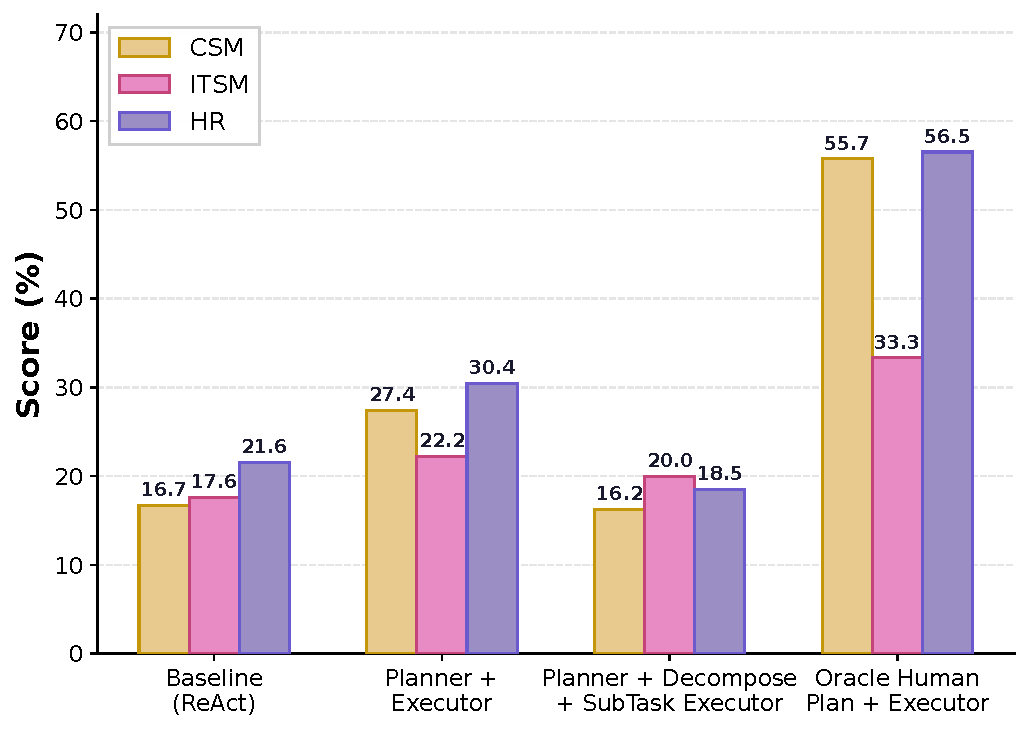
\includegraphics[width=1.0\linewidth]{figures/orchestrator_strategy_plot_overall.pdf}
 \caption{\textbf{智能体编排对性能的影响。}直方图给出采用 Claude-Sonnet-4.5 的不同多智能体架构性能。基线是第~\ref{subsec:baselines} 节描述的简单 ReAct 循环。\textit{规划器+执行器}架构先提示模型产生详细计划，再执行以该计划为条件的 ReAct 循环；\textit{规划器+分解+子任务执行器}进一步进行任务分解，并为每个子任务调用一个在 ReAct 循环中运行的子智能体；最后，\textit{预言式人工计划+执行器}以人工编写计划为条件执行 ReAct 循环。}
 \label{fig:mas_orchestration_analysis}
\end{figure}

\textbf{人工编写计划揭示了显著更高的上限。}为界定更好规划可能达到的效果，我们向相同执行器模型提供人工编写的参考计划，并要求其执行相应工具调用，从而完全解耦规划与执行。收益显著大于自动规划：跨模型和领域提升 14--35 个百分点，约为 Claude 生成计划所带来改进的两倍。值得注意的是，采用人工计划（以及 Claude 计划）的 Qwen3-4B 与相同条件下更大的模型相当，甚至超过它们。这表明，当战略性推理被外化后，剩余的主要挑战是忠实遵循指令和精确调用工具；无论规模如何，现代 LLM 在这两项能力上都展现了广泛的胜任力。这也可能说明，内部先验更强的大模型更倾向偏离给定计划，而较小模型会更字面地跟随逐步指令；当这些指令最优时，这反而是优势。然而，人工计划与 LLM 计划之间的差距表明，当前 LLM 在这些任务上的战略推理仍远未达到人类水平。

\textbf{更复杂的编排不能弥合这一差距。}我们针对 Claude Sonnet 4.5 评估两种 MAS 配置：一种\textit{规划器+执行器}系统，用自动生成的计划作为 ReAct 条件；另一种\textit{规划器+分解+子任务执行器}系统，额外分解任务，并为每个子任务调用单独的子智能体。我们将这些系统与有无人工编写计划的 ReAct 执行器基线比较。由图~\ref{fig:mas_orchestration_analysis} 可见，\textit{规划器+执行器}设置持续优于 ReAct 基线，在 CSM 和 HR 上分别绝对提升 10.7\% 和 8.8\%。但分解架构鲁棒性较弱：它虽在 ITSM 上有小幅提升，却在 CSM 和 HR 上退化，在 CSM 上甚至低于基础 ReAct（16.2\% 对 16.7\%）。这与 \ours{} 任务具有强顺序状态依赖、而分解会破坏这种依赖相一致。最终，自动系统与采用人工计划的 ReAct 之间仍然存在显著差距，说明进展需要约束感知计划生成，而非仅靠架构复杂度。

\paragraph{失败模式}
我们对模型取得部分进展却最终未完成任务的样本进行了人工定性分析，观察到若干反复出现的失败模式。模型经常在没有先查询必要先决条件的情况下调用创建数据库对象的工具，从而产生带有失效外键链接的悬空记录，称为\textbf{缺失先决条件查询}。例如，一个任务要求在特定类别下创建 HR 主题时，模型跳过检索可用类别，插入了孤立记录。当某些状态转移发生时，模型也无法触发系统策略规定的后续动作，称为\textbf{级联状态传播}失败。其他失败包括：不通过先前工具交互解析正确 ID 而把未经验证的标识符传给工具调用，称为\textbf{错误 ID 解析}；以及在尚未执行所有必要步骤前过早宣称任务完成，称为\textbf{过早完成幻觉}。为更系统地归类这些错误，我们使用 LLM（Claude Sonnet 4.5~\cite{claudeopus}）根据专家撰写的描述，将最终状态 SQL 验证器标记为三类：（i）\textit{任务完成}验证器检查是否实现主要用户目标；（ii）\textit{完整性约束}验证器检查系统是否保持一致状态与有效外键关系；（iii）\textit{权限与流程合规}验证器检查是否遵守管理权限和流程规则的系统策略。这些类别的验证器通过率见表~\ref{tab:verifier_analysis}。模型在\textit{权限与流程合规}上最为困难，这对现实部署尤其关键，因为策略违规会引发级联系统故障和严重的安全漏洞。
\begin{table}[htbp]
\centering
\resizebox{\columnwidth}{!}{%
\begin{tabular}{l|rr|rr|rr}
\hline
\multirow{2}{*}{\textbf{领域}} & \multicolumn{2}{c|}{\textbf{任务完成}} & \multicolumn{2}{c|}{\textbf{完整性约束}} & \multicolumn{2}{c}{\textbf{策略合规}} \\
& \textbf{样本数} & \textbf{分数} & \textbf{样本数} & \textbf{分数} & \textbf{样本数} & \textbf{分数} \\
\hline
Teams    & 100 & 82.3 & 20 & 90.0 & 8   & 81.3 \\
CSM      & 183 & 58.3 & 30 & 70.0 & 120 & 45.5 \\
Email    & 103 & 70.9 & 17 & 76.5 & 12  & 79.2 \\
ITSM     & 176 & 53.7 & 30 & 50.6 & 70  & 30.0 \\
Calendar & 104 & 71.5 & 8  & 62.5 & 19  & 76.1 \\
HR       & 182 & 63.2 & 47 & 56.0 & 94  & 50.4 \\
Drive    & 105 & 75.1 & 26 & 87.8 & 6   & 66.7 \\
Hybrid   & 152 & 60.0 & 23 & 72.5 & 18  & 61.1 \\
\hline
\end{tabular}
}
\caption{按类别统计的跨领域验证器通过率。模型在完整性约束（系统状态有效性）上得分最高，其次为任务完成；策略合规表现最低。各类别样本数不同；CSM、ITSM 和 HR 等负担更重的领域更强调完整性约束和策略合规。}
\label{tab:verifier_analysis}
\end{table}

